\documentclass[11pt,a4paper]{article}
\usepackage[utf8]{inputenc}
\usepackage[french]{babel}
\usepackage[T1]{fontenc}
\usepackage{amsmath}
\usepackage{amsfonts}
\usepackage{amssymb}
\usepackage{graphicx}
\usepackage{tikz}
\usepackage[left=2cm,right=2cm,top=2cm,bottom=2cm]{geometry}
\usepackage{hyperref}
\usepackage{float}
\usepackage{xcolor}
\usepackage{pgfplots}
\usepackage{asymptote}
\usepackage[european, straightvoltages, RPvoltages]{circuitikz}
\usetikzlibrary{babel}
\usepackage{siunitx}
\usepackage{wrapfig}
\usepackage{multicol} 
\usepackage{ulem}
\setlength{\parindent}{0pt}

\title{PROJET EIS - PX222}
\author{Guillemot MOUSSU et Rémi MAZZONE}
\date{2° semestre - 2022-2023}

\begin{document}
\maketitle
\tableofcontents
\listoffigures
\pagebreak

\section{Carnet de bord des séances}
\subsection{Séance 0 - 21/03/2023}
\subsubsection{Notes prises au tableau}
\begin{figure} [H]
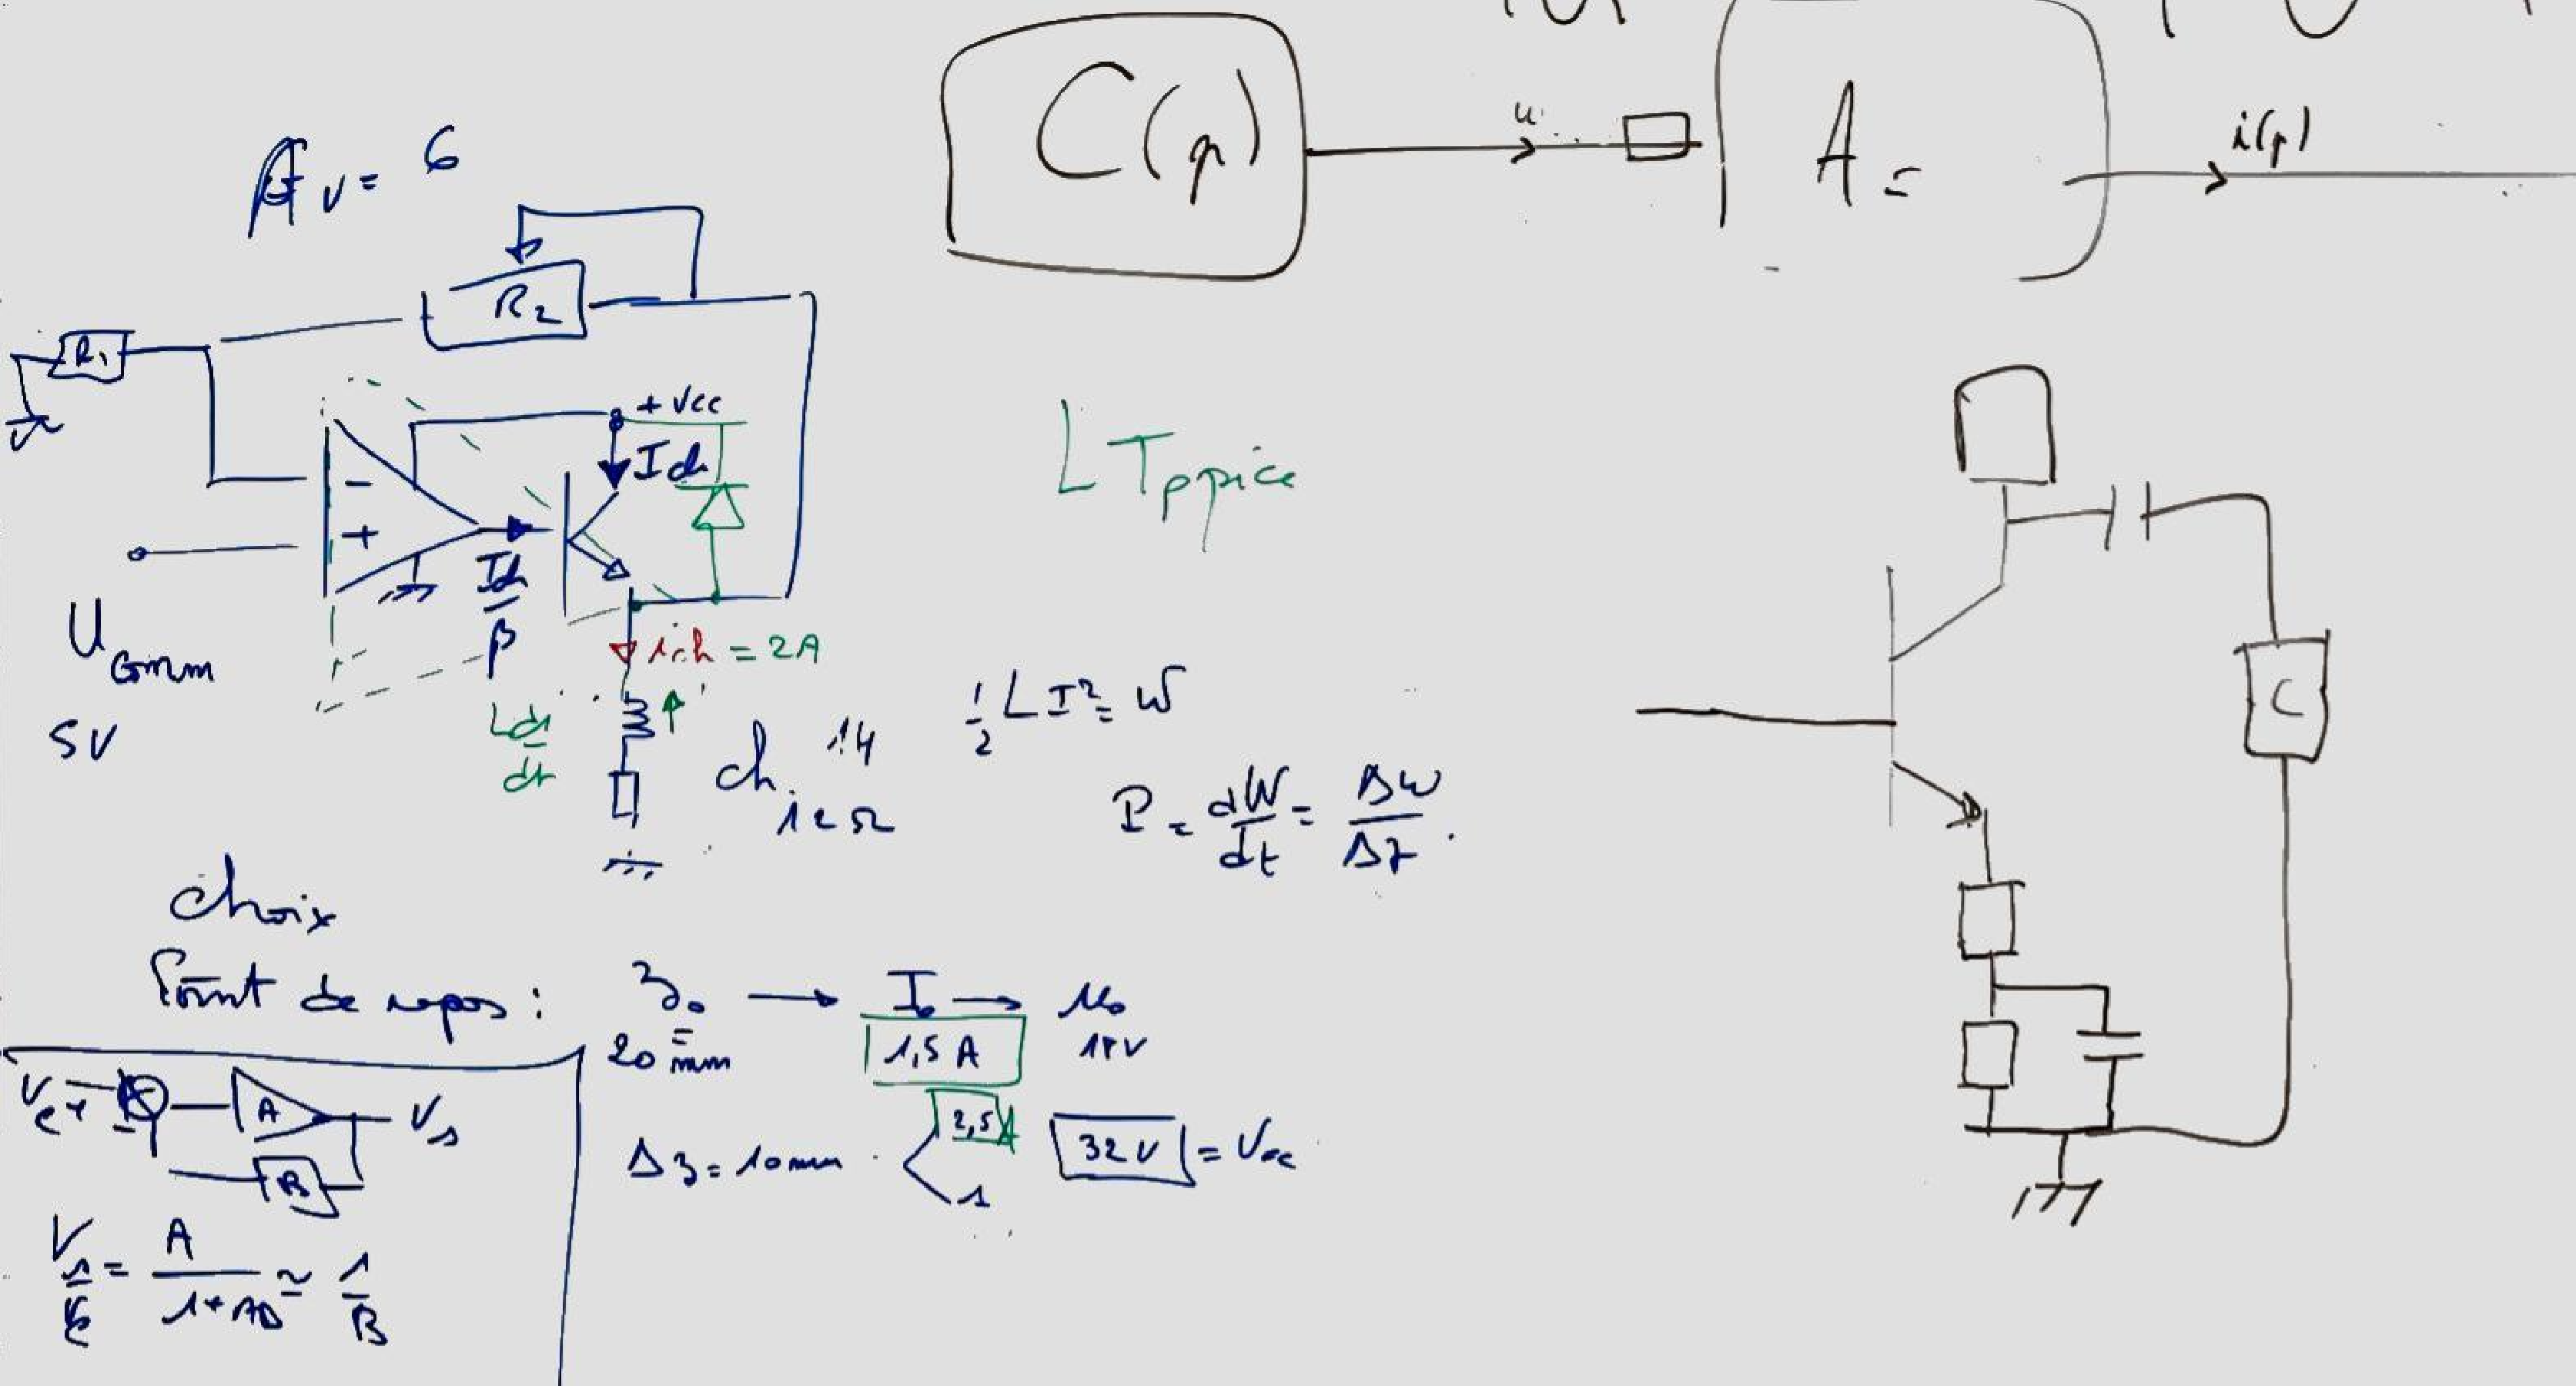
\includegraphics[width=1\textwidth]{Notes tableau séance 0.png} 
\caption{Notes séance 0}
\end{figure}

\subsubsection{Idées de plan de recherches}
\begin{itemize}
\item \textbf{Caractérisation de la bobine} : mesure de la résistance et l'inductance de la bobine. Cela permettra de modéliser la bobine et de calculer le champ magnétique qu'elle produit
\item \textbf{Modélisation de la bobine} : utilisation des valeurs mesurées pour construire un modèle électrique de la bobine, par exemple en utilisant l'équation de l'inductance d'une bobine. Pour une précision plus élevée, il peut être nécessaire d'inclure d'autres effets tels que la saturation du noyau de la bobine ou la résistance série équivalente
\item \textbf{Étude du champ magnétique de la bobine} : calcul de la distribution du champ magnétique à l'aide d'un logiciel de simulation. Validation des résultats expérimentalement
\item \textbf{Choix d'un capteur de distance} : choix d'un capteur de distance infrarouge adapté à la plage de mesure et à la précision requises. La fréquence de mesure et la plage de mesure peuvent influencer le résultat
\item \textbf{Calibration du capteur de distance} : déterminer la relation entre la tension de sortie du capteur et la distance de la bille par rapport à la bobine
\item \textbf{Conception d'un correcteur } : utiliser les données obtenues précédemment pour concevoir un correcteur proportionnel-intégral-dérivé (PID) ou un correcteur à avance de phase pour contrôler la position de la bille. C'est la partie clé de ce projet. Le correcteur PID est une méthode de contrôle classique qui est souvent utilisée pour les systèmes de positionnement. Un correcteur à avance de phase peut également être utilisé pour améliorer les performances.
\item \textbf{Implémentation du correcteur } : test du correcteur via Matlab et Simulink
\item \textbf{Étalonnage du système} : ajuster les paramètres du correcteur pour atteindre la précision et la stabilité requises
\item \textbf{Validation du système} : tester le système dans différentes conditions et valider ses performances
\item \textbf{Optimisation du système} : améliorer le système en optimisant les paramètres du correcteur et en utilisant des techniques avancées de contrôle, telles que le contrôle prédictif et le contrôle adaptatif
\end{itemize}
\medskip
Il est important de noter que certains des points ont déjà été réalisés lors du premier semestre

\subsection{Séance 1 - 05/04/2023}
\subsubsection{Reprise des éléments du semestre précédent}
Avec Hopkinson, nous avions obtenu un schéma équivalent de la bobine : 
\begin{figure}[H]
\begin{center}
\begin{circuitikz}
\draw
(0,0) to [V=$\varepsilon$] (0,2)
(0,2) to [short, i=$\varphi$] (2,2)
(2,2) to [R, l=$\mathfrak{R}_1$] (2,0)
(2,0) to [short] (0,0)
(2,2) to [R, l=$\mathfrak{R}(z)$, *-] (5,2)
(2,0) to [R, l=$\mathfrak{R}_0$, *-] (5,0)
(5,2) to [short] (5,0);
\end{circuitikz}
\caption{Modélisation de la bobine}
\end{center}
\end{figure}

Nous avions trouvé que la fonction de transfert de la bobine est : $\boxed{T_{BO}=\dfrac{Z}{I}=\dfrac{k_i}{k_z-mp^2}}$\\
Avec les valeurs suivantes :\\
\medskip
$I_0 = 2A$, $Z_0 = 22mm$, $L_1 = 6.73H$, $\alpha = 2.06$, $m = 35.8g$\\
$k_i = \dfrac{I_0 \cdot L_1 \cdot \alpha}{(1 + \alpha \cdot Z_0)^2}$, $k_z = \dfrac{I_0^2 \cdot L_1 \cdot \alpha^2}{(1 + \alpha \cdot Z_0)^3}$



\pagebreak
\section{Bibliographie}
Liste des sites utilisés pour la réalisation du projet :
\begin{itemize}
\item \href{https://www.overleaf.com/learn}{Overleaf, guide d'utilisation du \LaTeX{}}
\item \href{https://chat.openai.com/chat}{ChatGPT, modèle de langage automatisé}
\item \href{https://ctan.mines-albi.fr/graphics/pgf/contrib/circuitikz/doc/circuitikzmanual.pdf}{Manuel de Circuitikz}
\end{itemize}

\end{document}